\documentclass[preview]{standalone}
\usepackage{anyfontsize}
\usepackage{t1enc}
\usepackage{amsmath}
\usepackage{tcolorbox}
\usepackage{tikz}
\usepackage{amsfonts}
\usepackage{graphicx}
\usepackage{fancyhdr}
\usepackage{clrscode}
\usepackage{extramarks}
\usepackage{enumerate}
\usepackage{tkz-graph}

\usetikzlibrary{shapes.geometric, arrows, automata, positioning}

% golang colors
\definecolor{blue}{RGB}{55,94,171}
\definecolor{lblue}{RGB}{224,235,245}

% default sans
\renewcommand{\familydefault}{\sfdefault}

%%\fontencoding{T1}
%\fontfamily{calibri}
%%\fontseries{m}
%%\fontshape{it}
%\fontsize{28}{28}
%\selectfont

\tikzstyle{process} = [rectangle,
minimum width=2cm, minimum height=1.8cm,
text width=3.6cm, text centered,
draw=blue, fill=lblue]

\tikzstyle{arrow} = [ultra thick, ->, >=latex]


\begin{document}
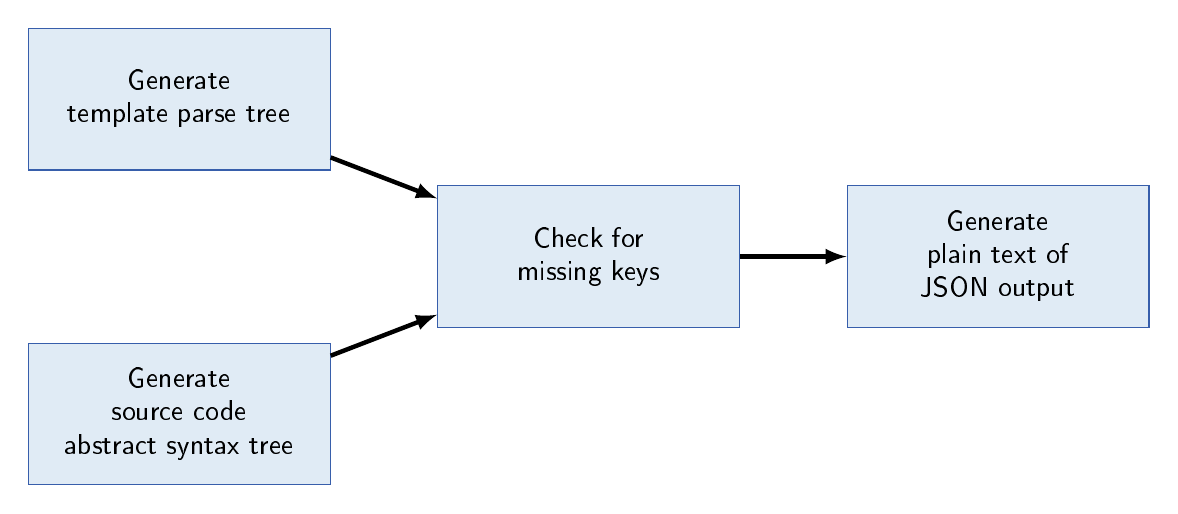
\begin{tikzpicture}[node distance=4cm]
    \GraphInit[vstyle=Normal] 
    \SetGraphUnit{3}
    \node (pro1) [process]
        {Generate \\ template parse tree};
    \node (pro2) [process, below of=pro1]
        {Generate \\ source code \\ abstract syntax tree};
    \node (pro3) [process, right of=pro2, xshift=1.2cm, yshift=2cm]
        {Check for \\ missing keys};
    \node (pro4) [process, right of=pro3, xshift=1.2cm]
        {Generate \\ plain text of \\ JSON output};

    \draw [arrow] (pro1) -- (pro3);
    \draw [arrow] (pro2) -- (pro3);
    \draw [arrow] (pro3) -- (pro4);
\end{tikzpicture}
\end{document}
